%%%%%%%%%%%%%%%%%%%%%%%%%%%%%%%%%%%%%%%%
% University/School Laboratory Report
% LaTeX Template
% Version 3.1 (25/3/14)
%
% This template has been downloaded from:
% http://www.LaTeXTemplates.com
%
% Original author:
% Linux and Unix Users Group at Virginia Tech Wiki 
% (https://vtluug.org/wiki/Example_LaTeX_chem_lab_report)
%
% License:
% CC BY-NC-SA 3.0 (http://creativecommons.org/licenses/by-nc-sa/3.0/)
%
%%%%%%%%%%%%%%%%%%%%%%%%%%%%%%%%%%%%%%%%%

%----------------------------------------------------------------------------------------
%   PACKAGES AND DOCUMENT CONFIGURATIONS
%----------------------------------------------------------------------------------------

\documentclass{article}

\usepackage[version=3]{mhchem} % Package for chemical equation typesetting
\usepackage{siunitx} % Provides the \SI{}{} and \si{} command for typesetting SI units
\usepackage{graphicx} % Required for the inclusion of images
\usepackage{natbib} % Required to change bibliography style to APA
\usepackage{amsmath} % Required for some math elements 
\usepackage{listings}
\usepackage{float}
\usepackage[center]{caption}
\usepackage{enumerate}
\usepackage{soul}

%\setlength\parindent{0pt} % Removes all indentation from paragraphs

%\renewcommand{\labelenumi}{\alph{enumi}.} % Make numbering in the enumerate environment by letter rather than number (e.g. section 6)

%\usepackage{times} % Uncomment to use the Times New Roman font

%----------------------------------------------------------------------------------------
%   DOCUMENT INFORMATION
%----------------------------------------------------------------------------------------

\date{\today} % Date for the report

\begin{document}

% Define document title and author
\title{Python Data Analysis}
\author{Johnny Pribyl}
\markboth{Montana State University}{}
\maketitle

\begin{abstract}
        This lab intends to provide an introduction to using Python as a tool
        for data analysis. Learning how to do basic statistics and plotting in
        Python makes it possible to leverage very powerful libraries. This week,
        I will be investigating SciPy, NumPy, and Matplotlib.
\end{abstract}



%----------------------------------------------------------------------------------------
%   SECTION 1
%----------------------------------------------------------------------------------------
\section{Introduction}

    This lab does not have an in-class portion. All you would need
    to reproduce the results is a computer with Python. I did all of my
    development in Vim. If you would like to emulate my environment, you can
    find my .vimrc on github at:

\begin{verbatim}
    jpribyl/legendary-waddle 
\end{verbatim}
Additionally, you can find all of my code at:
\begin{verbatim}
    jpribyl/cautious-palm-tree
\end{verbatim}

%----------------------------------------------------------------------------------------
%   SECTION 2
%----------------------------------------------------------------------------------------
\section{Starting Python}

I had a much easier time loading python than some of my peers.
While they had to mess around with the PATH and environment variables, I got to
sail off into the sunset by opening up a terminal and typing:
\begin{verbatim}
    python3
\end{verbatim}
It probably doesn't hurt that I have used Python before.

%----------------------------------------------------------------------------------------
%   SECTION 3
%----------------------------------------------------------------------------------------
\section{Python Primer}
There are no exercises in this section, so I don't have much to say about it. I
have used Spyder before, it's a very nice IDE. I've never used Python(x, y),
but I'm comfortable enough with package managers and the linux terminal that I
don't feel it is necessary.

%----------------------------------------------------------------------------------------
%   SECTION 4
%----------------------------------------------------------------------------------------
\section{Exercises: Python and Plotting}
\subsection{Numbers \& Arrays}
This section provides an extremely basic introduction to python. I think that
it's main purpose was to check whether my version of python supports implicit
conversion of integers to floats. (Spoiler, it does)

Sometimes I will accidentally set up a virtual environment in python 2.
However, I prefer using python 3. Among other things, it supports implicit
conversion of integers to floats. The code in this section was simple enough
that I opted to do input it directly to the terminal. Here are the results.
The characters $>>>$ occur before inputs but not before outputs.

\begin{verbatim}
    $ python3
    Python 3.5.2 
    [GCC 5.4.0 20160609] on linux
    >>> 5.0/3
    1.6666666666666667
    >>> 5/3
    1.6666666666666667
    >>> 5**2
    25
    >>> import numpy as np
    >>> np.sin(np.pi/6)
    0.49999999999999994
    >>> t=10
    >>> t2=2*t
    >>> g=-9.8
    >>> y=g*t**2/2
    >>> print(y)
    -490.00000000000006
\end{verbatim}
Had I tried using NumPy before importing it, I would have gotten an error:
\begin{verbatim}
    >>> np.pi
    Traceback (most recent call last):
     File "<stdin>", line 1, in <module>
    NameError: name 'np' is not defined
    >>> 
\end{verbatim}
Which could be good to keep in mind going forward.

\subsection{Plotting Data and Curves}
This section is a slight step up from the previous section. Although I do love
jupyter, I'm not quite ready to let go of vim, so I got familiar with 

\begin{lstlisting}
        plt.show()
\end{lstlisting}

The code for this section is detailed almost word for word in
$lab\_descrip/data\_analysis.pdf$ so I'm not going to recopy it here. If you go
to github, you can also find it in $simple\_plot.py$. 
\begin{figure}[H]
        % Center the figure.
        \begin{center}
        % Include the eps file, scale it such that it's width equals the column width. You can also put width=8cm for example...
        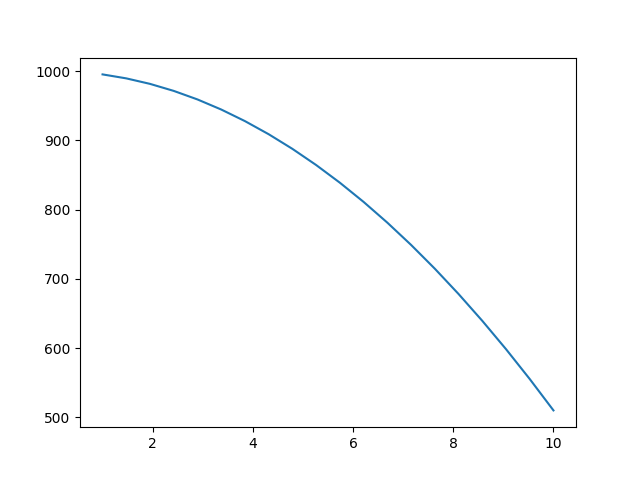
\includegraphics[width=6cm, height=6cm]{/home/jp/kod/py/bin/venv/py3/phx444/data_analysis/figures/figure1.png}
        % Create a subtitle for the figure.
        \caption{Simple plot of kinematics}
        % Define the label of the figure. It's good to use 'fig:title', so you know that the label belongs to a figure.
        \label{fig:fig_1}
        \end{center}
\end{figure}

If we alter the code a little bit, then we can easily include error bars, label axes, add a legend, change the
color, symbol, size, and line type. 
\begin{center}
\begin{minipage}[t]{.70\linewidth}
\begin{lstlisting}[caption=Altering the Graphs, frame=tlrb]{name}
# changing color, size, and symbol
plt.plot(
        t_theory,
        y_theory,
        'r.',
        MarkerSize=1
)

# labelling axes
plt.xlabel('time (s)')
plt.ylabel('height (m)')

# and, adding a legend
plt.legend(['Theory', 'Actual'])
plt.show()
plt.savefig('figures/figure3.png')

\end{lstlisting}
\end{minipage}
\end{center}


And produce this plot:
\begin{figure}[H]
        % Center the figure.
        \begin{center}
        % Include the eps file, scale it such that it's width equals the column width. You can also put width=8cm for example...
        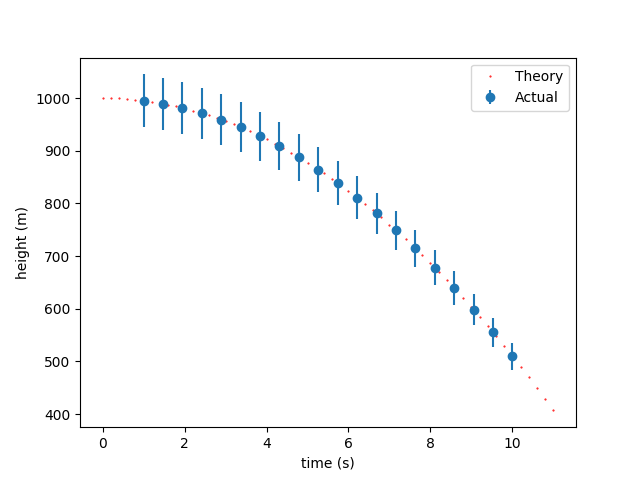
\includegraphics[width=6cm, height=6cm]{/home/jp/kod/py/bin/venv/py3/phx444/data_analysis/figures/figure3.png}
        % Create a subtitle for the figure.
        \caption{Changing size and introducing a legend}
        % Define the label of the figure. It's good to use 'fig:title', so you know that the label belongs to a figure.
        \label{fig:fig_3}
        \end{center}
\end{figure}

\subsection{Example of Input/Output}
I decided to do this all in one script. It seemed to work just fine for me, but
if you run into any issues, you can definitely split it apart into two
scripts. The idea is to save an array into a file and then read it back and
plot the results. Here is my script:

\begin{center}
\begin{minipage}[t]{.80\textwidth}
\begin{lstlisting}[caption=Input / Output, frame=tlrb]
import numpy as np
import matplotlib.pyplot as plt

x = np.linspace(0, 10, 50)
y = np.exp(-x)

data_out = np.column_stack((x, y))
np.savetxt('output.dat', data_out)

u, v = np.loadtxt('output.dat', unpack=True)
plt.plot(u, v)
plt.xlabel('Dummy Label')
plt.ylabel('Dummy Label')
plt.savefig('figures/figure4')
plt.show()
\end{lstlisting}
\end{minipage}
\end{center}

And the plot that it produces:
\begin{figure}[H]
        % Center the figure.
        \begin{center}
        % Include the eps file, scale it such that it's width equals the column width. You can also put width=8cm for example...
        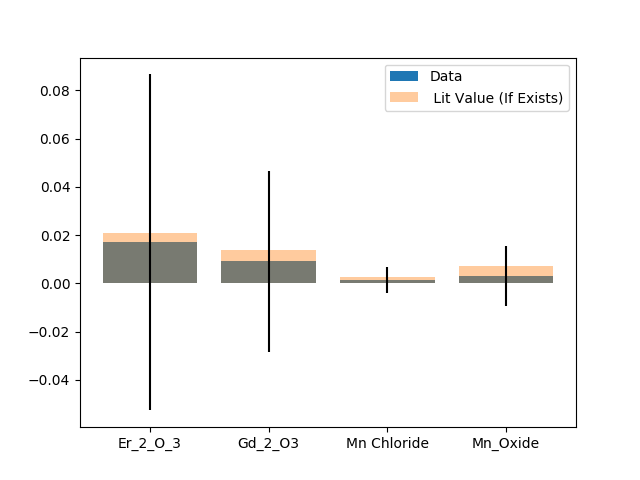
\includegraphics[width=6cm, height=6cm]{/home/jp/kod/py/bin/venv/py3/phx444/data_analysis/figures/figure4.png}
        % Create a subtitle for the figure.
        \caption{Reading points out of a saved np.array}
        % Define the label of the figure. It's good to use 'fig:title', so you know that the label belongs to a figure.
        \label{fig:fig_4}
        \end{center}
\end{figure}

%----------------------------------------------------------------------------------------
%   SECTION 5
%----------------------------------------------------------------------------------------
\section{Exercises: Analysis using Simple functions}
Here I will use NumPy, and Matplotlib to plot some simple functions. The
accompanying code may be found in $simple\_functions.py$.

\subsection{Linear and Quadratic Functions}
As a general rule, it is stylistically better to define functions and classes
instead of tossing everything int a single script. However, the exercises in
this week's lab were simle enough that it was not entirely necessary, so I did
not bother


\subsubsection{Linear Plotting}

We are asked to plot a simpe linear function and fiddle with the
graph limits and tick marks. I'm not going to include the graph for
this exercise, but it will be obvious going forward that I did, in
fact, plot it. Additionally, here are the methods that you shoud use if
you are following along with your morning coffee and totally stumped.

\begin{center}
\begin{minipage}[t]{.80\textwidth}
\begin{lstlisting}[caption=Limits \& Ticks, frame=tlrb]
plt.xlim(-15, 15)
plt.ylim(-15, 15)

plt.xticks(whatever you want in here)
plt.yticks(maybe a range(0,10) or something)
\end{lstlisting}
\end{minipage}
\end{center}

\subsubsection{Perpendicular Lines}
In the previous section, we plotted a line with a slope of 2. So, if you
squint at that for a while and tilt your head, you might eventually throw in the
towel and accept that a line with a slope of $- 1/2$ is perpendicular to it.

We can use the results of the previous section to ensure that both axes have
the same scale, and plot the results on a single graph:
\begin{figure}[H]
        % Center the figure.
        \begin{center}
        % Include the eps file, scale it such that it's width equals the column width. You can also put width=8cm for example...
        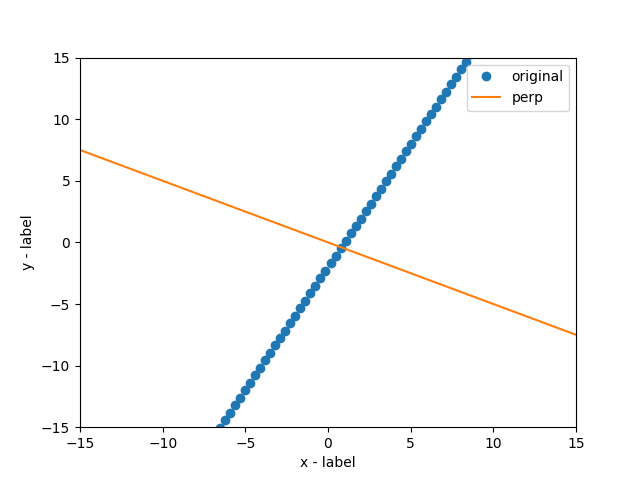
\includegraphics[width=6cm,
        height=6cm]{/home/jp/kod/py/bin/venv/py3/phx444/data_analysis/figures/exercise2.png}
        % Create a subtitle for the figure.
        \caption{These lines have a vanishing dot product!}
        % Define the label of the figure. It's good to use 'fig:title', so you know that the label belongs to a figure.
        \label{fig:fig_5}
        \end{center}
\end{figure}

\subsubsection{Simplest Quadratic}
I hope every lab includes a graph like this. Using:

\begin{center}
\begin{minipage}[t]{.75\textwidth}
    \begin{lstlisting}[caption= Just in Case, frame=tlrb]
y = x**2
plt.xlim(-5,5)
plt.plot(x, y)
plt.xlabel('x - label')
plt.ylabel('y - label')
\end{lstlisting}
\end{minipage}
\end{center}
We find:
\begin{figure}[H]
        % Center the figure.
        \begin{center}
        % Include the eps file, scale it such that it's width equals the column width. You can also put width=8cm for example...
        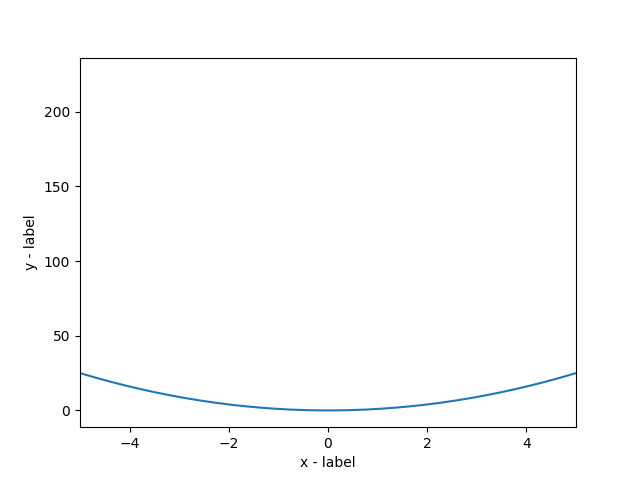
\includegraphics[width=6cm,
        height=6cm]{/home/jp/kod/py/bin/venv/py3/phx444/data_analysis/figures/exercise3.png}
        % Create a subtitle for the figure.
        \caption{The very simple-est quadratic}
        % Define the label of the figure. It's good to use 'fig:title', so you know that the label belongs to a figure.
        \label{fig:fig_6}
        \end{center}
\end{figure}

\subsubsection{But, What does it Mean?}
By experiment and the scientific method, I was able to deduce that $x_0$
controls the x-value for the base of the parabola, $y_0$ controls the y-value
for the base of the parabola, and a controls the slope of the parabola's sides.
Check it out!

\begin{figure}[H]
        % Center the figure.
        \begin{center}
        % Include the eps file, scale it such that it's width equals the column width. You can also put width=8cm for example...
        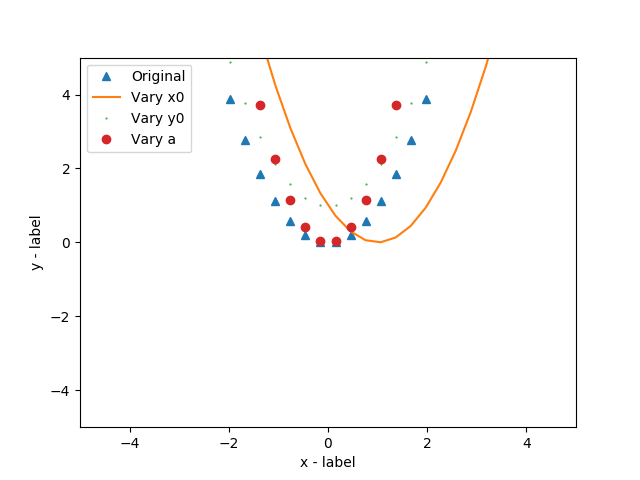
\includegraphics[width=6cm,
        height=6cm]{/home/jp/kod/py/bin/venv/py3/phx444/data_analysis/figures/exercise4.png}
        % Create a subtitle for the figure.
        \caption{Play with the constants, the scale, and the ticks. Especially
            the ticks. They love the attention.}
        % Define the label of the figure. It's good to use 'fig:title', so you know that the label belongs to a figure.
        \label{fig:fig_7}
        \end{center}
\end{figure}

\subsubsection{Projectile Motion}

Here we are asked to examine projectile motion with no resistance. These
equations should look familiar. I solved the initial conditions for $V_{0x}
~\& ~ V_{0y}$ and plugged those in as well.

\begin{center}
\begin{minipage}[t]{.75\textwidth}
\begin{lstlisting}[frame=tlrb]
plt.clf()
x0 = 0
y0 = 0
g = 9.81

# solving the equation for 25 degrees
v0x = 54.3785
v0y = 25.3571

t = np.linspace(0, 5, 50)

y = v0y * t - 1 / 2 * g * t ** 2

x = v0x * t 

# angle is np.arctan( v0y / v0x )
# np.sqrt(v0x ** 2 + v0y ** 2) = 60

plt.xlabel('distance (meters)')
plt.ylabel('height (meters)')
plt.plot(x, y)
plt.legend()
plt.savefig('figures/exercise5')

\end{lstlisting}
\end{minipage}
\end{center}

And here is the plot:


\begin{figure}[H]
        % Center the figure.
        \begin{center}
        % Include the eps file, scale it such that it's width equals the column width. You can also put width=8cm for example...
        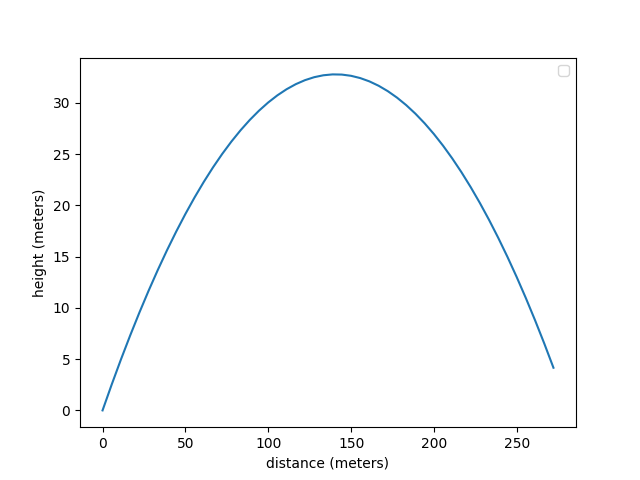
\includegraphics[width=6cm,
        height=6cm]{/home/jp/kod/py/bin/venv/py3/phx444/data_analysis/figures/exercise5.png}
        % Create a subtitle for the figure.
        \caption{Projectiles flying, through the air}
        % Define the label of the figure. It's good to use 'fig:title', so you know that the label belongs to a figure.
        \label{fig:fig_8}
        \end{center}
\end{figure}

\subsubsection{$\frac{\pi}{4}$ Flies the Furthest}
This is pretty straightforward. I plotted three trajectories. One is at 45
degrees, another is slightly above, and the last one is slightly below. I used
mathematica to solve the system for my three sets of initial conditions. You
could do it in Python, but Mathematica is really way better at algebra. So,
it's worth using in this case.


\begin{figure}[H]
        % Center the figure.
        \begin{center}
        % Include the eps file, scale it such that it's width equals the column width. You can also put width=8cm for example...
        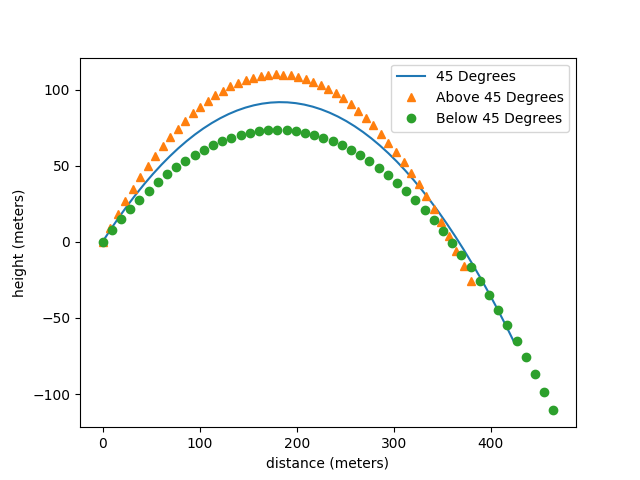
\includegraphics[width=6cm,
        height=6cm]{/home/jp/kod/py/bin/venv/py3/phx444/data_analysis/figures/exercise6a.png}
        % Create a subtitle for the figure.
        \caption{Experimenting with Initial Conditions}
        % Define the label of the figure. It's good to use 'fig:title', so you know that the label belongs to a figure.
        \label{fig:fig_9}
        \end{center}
\end{figure}

That plot really does a pretty awful job of showing where the flying particles
land with respect to each other. But, we can zoom in on the point.


\begin{figure}[H]
        % Center the figure.
        \begin{center}
        % Include the eps file, scale it such that it's width equals the column width. You can also put width=8cm for example...
        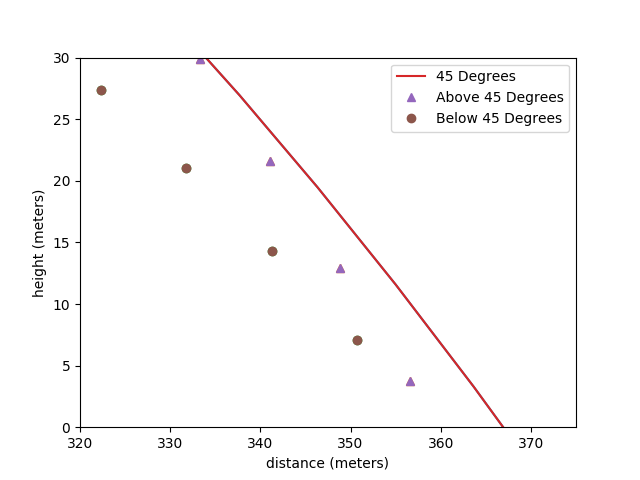
\includegraphics[width=6cm,
        height=6cm]{/home/jp/kod/py/bin/venv/py3/phx444/data_analysis/figures/exercise6b.png}
        % Create a subtitle for the figure.
        \caption{Proving that $\frac{\pi}{4}$ will make things go far}
        % Define the label of the figure. It's good to use 'fig:title', so you know that the label belongs to a figure.
        \label{fig:fig_10}
        \end{center}
\end{figure}

And we find, as expected, the line at 45 degrees travels the farthest distance.

\subsection{Exponential Funtions}
There is a very special number in the universe. We call it "e" for some reason.
Probably historical.

\subsubsection{Plot the Exponential Function}
First things first. Let's see what this "e" thing looks like.

\begin{figure}[H]
        % Center the figure.
        \begin{center}
        % Include the eps file, scale it such that it's width equals the column width. You can also put width=8cm for example...
        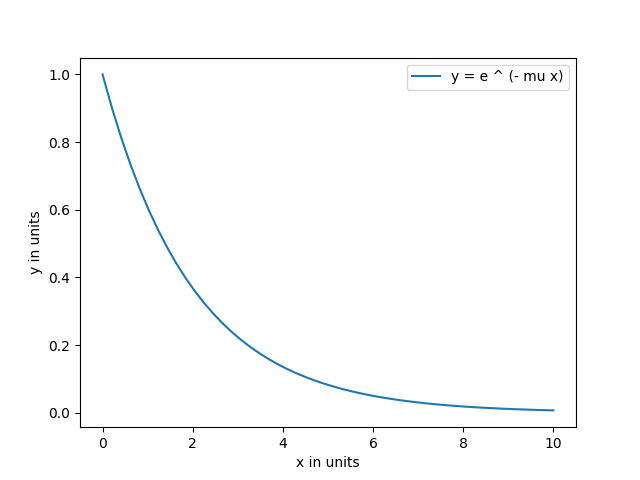
\includegraphics[width=6cm,
        height=6cm]{/home/jp/kod/py/bin/venv/py3/phx444/data_analysis/figures/exponential.png}
        % Create a subtitle for the figure.
        \caption{What does "e" look like?}
        % Define the label of the figure. It's good to use 'fig:title', so you know that the label belongs to a figure.
        \label{fig:fig_11}
        \end{center}
\end{figure}

And now, let's make the y-axis logarithmic with

\begin{center}
\begin{minipage}[t]{.75\textwidth}
\begin{lstlisting}[frame=tlrb]
plt.yscale('log')
\end{lstlisting}
\end{minipage}
\end{center}
\begin{figure}[H]
        \begin{center}
        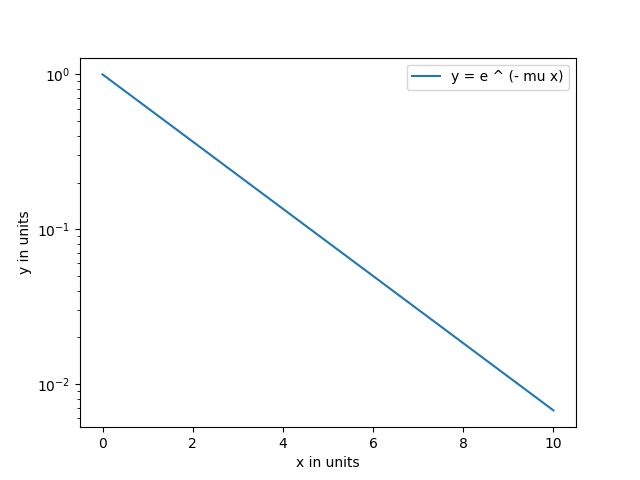
\includegraphics[width=6cm,
        height=6cm]{/home/jp/kod/py/bin/venv/py3/phx444/data_analysis/figures/exponential_log.png}
        \caption{Log-log-logarithms!}
        \label{fig:fig_12}
        \end{center}
\end{figure}

And we see that $\mu$ is acutally $\frac{1}{slope}$ on a logarithmic scale. You
could also see this by taking the natural log of boths sides and doing math.

\subsubsection{Exponential Decay and RC Circuits}
In the case of exponential decay, $\mu$ is called a "decay rate" and is related
to how fast the decay occurs. In the circuit, $\mu$ is the inverse of the time
constant. The time constant $\tau$ controls how quickly voltage will fall in a
system.

\subsection{Gaussian Function}
Another thing that seems to show up everywhere in this universe is the so
called "normal" distribution. It's also called a Gaussian.

\subsubsection{Normalize and Plot}
Normalizing a gaussian means that it integrates to one over the interval from
negative infinity to positive infinity. Typically, we normalize a gaussian any
time that it corresponds to a probability distribuion. Following along with the
appendix, this was not too hard to do in Python. We can also play around with
the mean and the standard deviation. We'll see momentarily that a lower
standard deviation corresponds to a narrower envelope
\begin{center}
\begin{minipage}[t]{.85\textwidth}
\begin{lstlisting}[frame=tlrb]
x = np.linspace(-6, 6, 150)

def gaussian(x, N0, mu, sigma):
    return N0*np.exp(-0.5*((x-mu)/sigma)**2)

sigma = 2
mu = 0
N0 = 1 / ( sigma * np.sqrt(2 * np.pi) )
f = gaussian(x, N0, mu, sigma)
g = gaussian(x, N0, mu + 1, sigma / 2)

plt.plot(x, f,label='original')
plt.plot(x, g,'o', markersize=1, label='shifted')
plt.legend()
# plt.show()
plt.savefig('figures/gaussian.png')
\end{lstlisting}
\end{minipage}
\end{center}

Or, graphically
\begin{figure}[H]
        % Center the figure.
        \begin{center}
        % Include the eps file, scale it such that it's width equals the column width. You can also put width=8cm for example...
        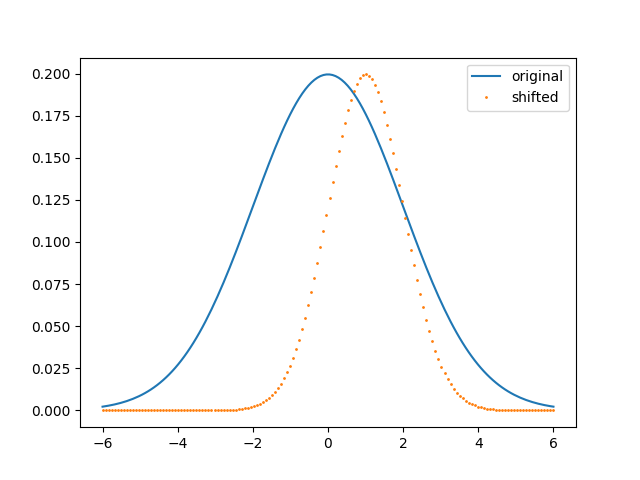
\includegraphics[width=6cm,
        height=6cm]{/home/jp/kod/py/bin/venv/py3/phx444/data_analysis/figures/gaussian.png}
        % Create a subtitle for the figure.
        \caption{Plotting a Normalized Gaussian}
        % Define the label of the figure. It's good to use 'fig:title', so you know that the label belongs to a figure.
        \label{fig:fig_13}
        \end{center}
\end{figure}

\subsubsection{Using 'Quad' to Integrate}
A moment ago, we discussed normalization. But let's see if our gaussian really
IS normalized. 

\begin{center}
\begin{minipage}[t]{.75\textwidth}
\begin{lstlisting}[frame=tlrb]
inf = 10 * sigma
lower_bound = - inf
upper_bound = inf

I = quad(
    gaussian,
    lower_bound,
    upper_bound,
    args=(N0, mu, sigma)
)

print(I)

\end{lstlisting}
\end{minipage}
\end{center}

You'll have to take my word that it works.

\subsubsection{Use the Definition of the Mean..}
We also discussed the mean, $\mu$, of the gaussian. So let's use the definition
of the mean:
$$\mu = \frac{\int_{-\infty}^{\infty x f(x) dx}}{\int_{-\infty}^{\infty} f(x) dx}$$
Or, in Python

\begin{center}
\begin{minipage}[t]{.75\textwidth}
\begin{lstlisting}[frame=tlrb]
def x_gauss(x, N0, mu, sigma):
    return x * N0*np.exp(
        -0.5*((x-mu)/sigma)**2)

J = quad(
    x_gauss,
    lower_bound,
    upper_bound,
    args=(N0, mu, sigma)
)

\end{lstlisting}
\end{minipage}
\end{center}

And we do, in fact get back 0.

\subsubsection{More Integration}
Brian's curiosity is insatiable. Now we are integrating from $-\infty
\rightarrow x - \sigma$ and then from $x + \sigma \rightarrow \infty $in order to demonstrate that
statistics work. Converting this into Python we find:
\begin{center}
\begin{minipage}[t]{.80\textwidth}
\begin{lstlisting}[frame=tlrb]
lower_bound = - inf
upper_bound = mu - sigma
below_envelope = quad(
    gaussian,
    lower_bound,
    upper_bound,
    args=(N0, mu, sigma)
)

lower_bound = mu + sigma
upper_bound = inf
above_envelope = quad(
    gaussian,
    lower_bound,
    upper_bound,
    args=(N0, mu, sigma)
)

print(below_envelope[0] + above_envelope[0])

\end{lstlisting}
\end{minipage}
\end{center}
Again, you'll have to take my word for it, but it comes out to right around
32\%

\section{Statistical Analysis}
This is where things start to get interesting. Bear with me, there are only 14
exercises left.

\subsection{Errors, Means, and Standard Deviations}
There's some interesting theory in this section that I'm not going to recopy,
but it is worth glancing over. Especially if you've never taken statistics. 

\subsubsection{Find the Mean and Std of a Sample Data Set}
Here we have a nice data set with 25 points. I decided to toss this into an
array, because of broadcasting. And other NumPy reasons.
\begin{center}
\begin{minipage}[t]{.75\textwidth}
\begin{lstlisting}[frame=tlrb]
ds = np.array(
    [
        212.3,
        211.5,
        210.8,
        209.8,
        211.1,
        210.6,
        213.2,
        211.7,
        212.6,
        210.3,
        212.1,
        211.5,
        210.6,
        213.0,
        212.1,
        211.7,
        212.1,
        211.3,
        211.8,
        211.4,
        213.4,
        210.5,
        211.0,
        211.1,
        212.7
    ]
)
mean = np.mean(ds)
std = np.std(ds)
b = np.linspace(205, 220, 49)

print(mean)
print(std)
print(ds)

\end{lstlisting}
\end{minipage}
\end{center}

Since you can't just type $<$leader$>$b to see the output, I guess I'll transcribe
it. The mean comes out to 211.608 and the standard deviation is 0.9178.

\subsubsection{Histogram Plotting}

Here we are asked to turn these points into a histogram using plt.hist.
\begin{center}
\begin{minipage}[t]{.75\textwidth}
\begin{lstlisting}[frame=tlrb]
plt.hist(
    ds,
    bins=b,
    #density=True,
    label='Measured'
)

plt.xlabel('Table Length in Cm')

plt.ylabel(
    'Number of measurements
    (Normalized to 1)'
)
plt.yticks(range(0,5))

\end{lstlisting}
\end{minipage}
\end{center}

Which produces this:

\begin{figure}[H]
        % Center the figure.
        \begin{center}
        % Include the eps file, scale it such that it's width equals the column width. You can also put width=8cm for example...
        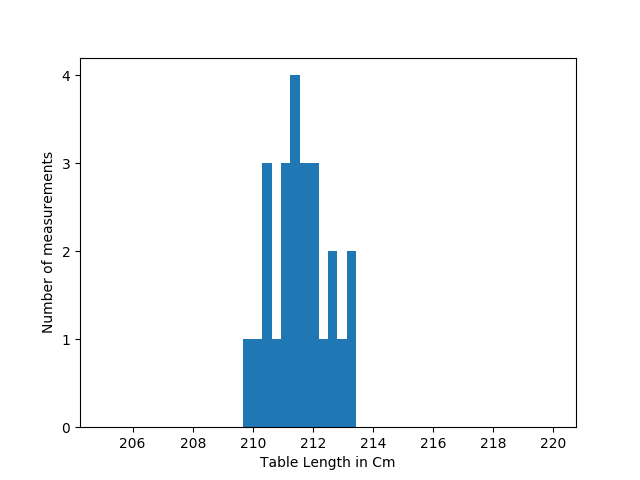
\includegraphics[width=6cm,
        height=6cm]{/home/jp/kod/py/bin/venv/py3/phx444/data_analysis/figures/612.png}
        % Create a subtitle for the figure.
        \caption{Plotting a Histgram}
        % Define the label of the figure. It's good to use 'fig:title', so you know that the label belongs to a figure.
        \label{fig:fig_14}
        \end{center}
\end{figure}

\subsubsection{Superimposing a Gaussian}
Sometimes a histogram just doesn't quite cut it. So, we can normalize the
histogram and then superimpose a normalized gaussian over it to see visually
whether they match. Normalizing an array is actually pretty easy in python. All
you have to do is uncomment the 'density=True' in my code up there. Then you
can define a gaussian just like we did earlier. In case your memory is as bad
as mine, we did it like this:

\begin{center}
\begin{minipage}[t]{.80\textwidth}
\begin{lstlisting}[frame=tlrb]
x = np.linspace(205,220,200)

def gaussian(x, mu, sigma):
    N0 = 1 / ( sigma * np.sqrt(2 * np.pi) )
    return N0*np.exp(-0.5*((x-mu)/sigma)**2)

gauss = gaussian(x, mean, std)

plt.plot(
    x,
    gauss,
    label='Gaussian from Sample Mean and Std'
)
\end{lstlisting}
\end{minipage}
\end{center}

And you will see that these points are actually pretty normal:
\begin{figure}[H]
        % Center the figure.
        \begin{center}
        % Include the eps file, scale it such that it's width equals the column width. You can also put width=8cm for example...
        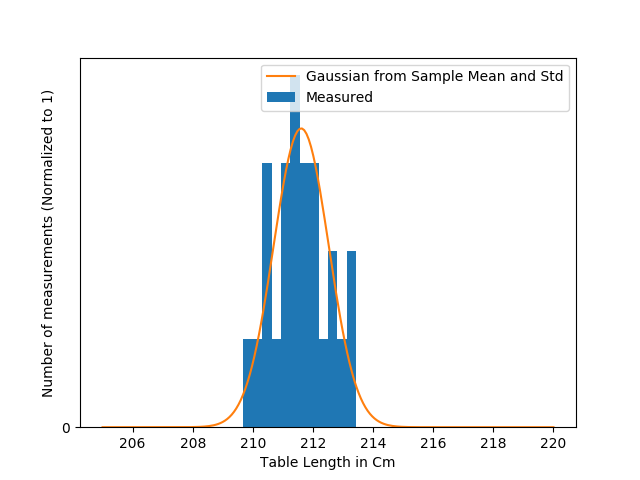
\includegraphics[width=6cm,
        height=6cm]{/home/jp/kod/py/bin/venv/py3/phx444/data_analysis/figures/613.png}
        % Create a subtitle for the figure.
        \caption{Superimposing a Gaussian on Normalized Data}
        % Define the label of the figure. It's good to use 'fig:title', so you know that the label belongs to a figure.
        \label{fig:fig_15}
        \end{center}
\end{figure}

\subsubsection{Leveraging NumPy}
But, why would we do all the heavy statistical lifting? You know, things like
finding a mean... or a standard deviation. That's just silly! Let's have SciPy
do it all for us with norm.fit.

\begin{center}
\begin{minipage}[t]{.75\textwidth}
\begin{lstlisting}[frame=tlrb]
mu_fit, sigma_fit = norm.fit(ds)
gauss_fit = gaussian(x, mu_fit, sigma_fit)

plt.plot(
    x,
    gauss_fit,
    '.',
    label='Gaussian Fit'
)

plt.legend()
plt.show()

\end{lstlisting}
\end{minipage}
\end{center}

And we see that the results are identical:
\begin{figure}[H]
        % Center the figure.
        \begin{center}
        % Include the eps file, scale it such that it's width equals the column width. You can also put width=8cm for example...
        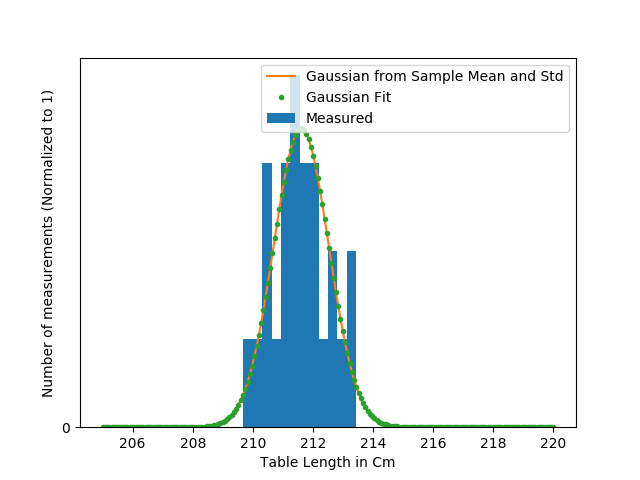
\includegraphics[width=6cm,
        height=6cm]{/home/jp/kod/py/bin/venv/py3/phx444/data_analysis/figures/614.png}
        % Create a subtitle for the figure.
        \caption{Super Superimposing a SciPy Gaussian on a Manual Gaussian on a
            Histogram. Don't worry, everything's normalized}
        % Define the label of the figure. It's good to use 'fig:title', so you know that the label belongs to a figure.
        \label{fig:fig_16}
        \end{center}
\end{figure}

\subsection{Error Propagation}
From chatting with Jennifer, it sounds like error propagation is very likely
going to be one of the trickiest things we do this semester. Maybe we should do
some exercises on it. I don't have a copy of Hughes and Hase. Besides, I'm
illeterate.

\subsection{Curve Fitting}
Getting away from Error Propagation, let's fit some curves! That will be fun.

\subsubsection{Experimental Data}
When I was in kindergarten, My Very Educated Mother Just Served Us Nine Pizzas.
Later we found out the Pizzas were actually Nachos, and nobody is really quite
sure how many Nachos we were served. The only thing we know for certain at this
point is that Brian just served us twelve new data points. I'm not going to
recopy them here, but you can find them in the lab if you're curious and not
finished with your coffee yet.

\subsubsection{Plotting Our Twelve Data Points}
Well, let's do some guestimating. I guestimate a slope of -4.0 and a y
intercept of 14.
\begin{center}
\begin{minipage}[t]{.80\textwidth}
\begin{lstlisting}[frame=tlrb]
plt.errorbar(
    x,
    y,
    fmt='.',
    yerr=y_err,
    label='measured points'
)

x_est = np.linspace(-2, 9, 50)
y_est = -4.0 * x_est + 14
plt.plot(x_est, y_est, label='estimated fit')
\end{lstlisting}
\end{minipage}
\end{center}

And it looks pretty good:
\begin{figure}[H]
        % Center the figure.
        \begin{center}
        % Include the eps file, scale it such that it's width equals the column width. You can also put width=8cm for example...
        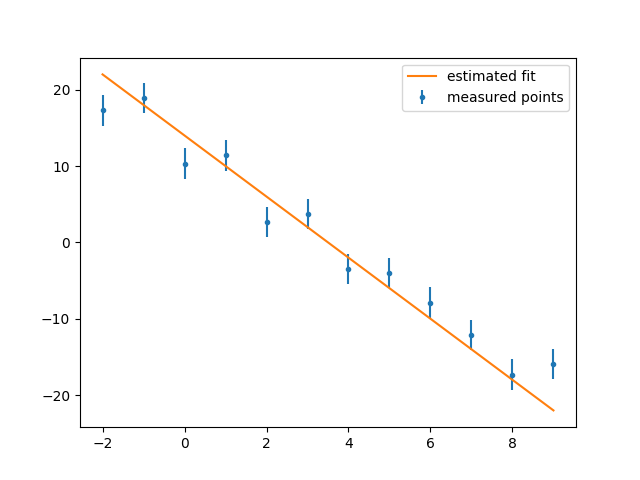
\includegraphics[width=6cm,
        height=6cm]{/home/jp/kod/py/bin/venv/py3/phx444/data_analysis/figures/622.png}
        % Create a subtitle for the figure.
        \caption{Plotting the data set and guessing at a fit}
        % Define the label of the figure. It's good to use 'fig:title', so you know that the label belongs to a figure.
        \label{fig:fig_17}
        \end{center}
\end{figure}

\subsubsection{Doing a Math}
Instead of fitting points with a ruler, we can use SciPy to do it! It's pretty
easy if you follow along in the appendix.

\begin{center}
\begin{minipage}[t]{.75\textwidth}
\begin{lstlisting}[frame=tlrb]
def func_to_fit(x, a, b):
    return a*x + b

popt, pcov = curve_fit(
    func_to_fit,
    x,
    y,
    sigma=y_err,
    p0=None
)

y_fit = func_to_fit(x, *popt)

plt.plot(
    x_est,
    func_to_fit(x_est, *popt),
    '.r',
    label='curve_fit'
)

plt.plot(x, y_fit)
plt.xlabel('x - data')
plt.ylabel('y - data')
\end{lstlisting}
\end{minipage}
\end{center}
And plotting this, it even seems to work:
\begin{figure}[H]
        % Center the figure.
        \begin{center}
        % Include the eps file, scale it such that it's width equals the column width. You can also put width=8cm for example...
        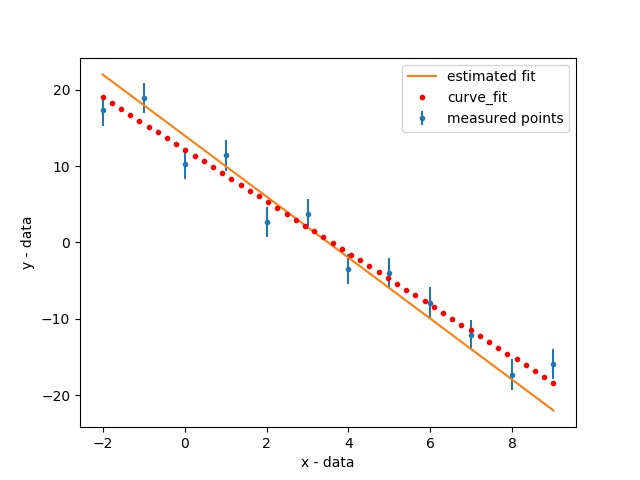
\includegraphics[width=6cm,
        height=6cm]{/home/jp/kod/py/bin/venv/py3/phx444/data_analysis/figures/623.png}
        % Create a subtitle for the figure.
        \caption{Using SciPy to fit a curve}
        % Define the label of the figure. It's good to use 'fig:title', so you know that the label belongs to a figure.
        \label{fig:fig_18}
        \end{center}
\end{figure}

\subsubsection{Qualitative Analysis}
I qualitatively analyze that my curve\_fit function is plotted in little red
bullet points. But not for you. For you they're grey. I strongly disagree with
the spelling of that word. As we discussed previously, there are 12 points. My
estimated fit goes through $\frac{7}{12}$ of those points. That's not quite as
good as the curve\_fit function which goes through $\frac{8}{12}$ of them.
$\frac{8}{12}$ is the same is $\frac{2}{3}$. That means we got a good fit. 

\subsubsection{Quantitative Analysis}
If we want to know exactly how good our fit is, then we can use $\chi^2$.
Following along with the appendix again, we can translate the definition into
Python

\begin{center}
\begin{minipage}[t]{.85\textwidth}
    \begin{verbatim}
chi2 = 
    np.sum(((y-func_to_fit(x, *popt))/y_err)**2) / (12 - 2)
\end{verbatim}
\end{minipage}
\end{center}

Printing this out, we get a $\chi^2$ value of 1.28.

\subsubsection{Eyeball Uncertainty}
Better plot this one.
\begin{figure}[H]
        % Center the figure.
        \begin{center}
        % Include the eps file, scale it such that it's width equals the column width. You can also put width=8cm for example...
        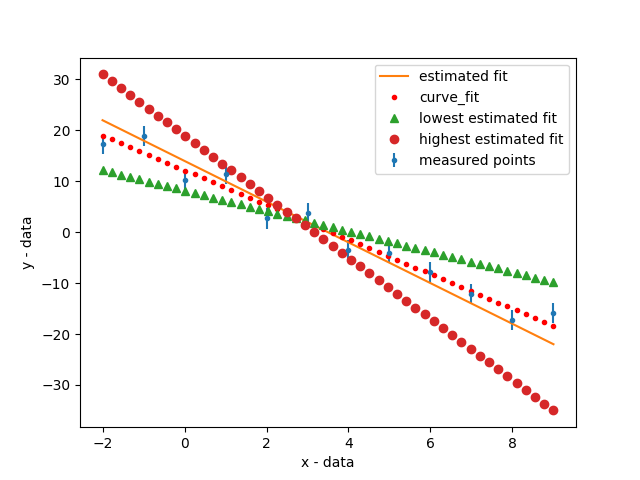
\includegraphics[width=6cm,
        height=6cm]{/home/jp/kod/py/bin/venv/py3/phx444/data_analysis/figures/626.png}
        % Create a subtitle for the figure.
        \caption{Eyeballing Uncertainty}
        % Define the label of the figure. It's good to use 'fig:title', so you know that the label belongs to a figure.
        \label{fig:fig_19}
        \end{center}
\end{figure}

My upper line has a slope of -6 and a y-intercept of 19 while my lower line has
a slope of -2 and a y-intercept of 8.2. Doing some back of the envelope math,
this means my uncertainty in the slope is $\pm2$ and my intercept is $~\pm5.5$.

\subsubsection{Quantitative Uncertainties}

I really love when you can do things in one line with Python. That always makes
me so happy.

\begin{center}
\begin{minipage}[t]{.80\textwidth}
\begin{lstlisting}[frame=tlrb]
parameter_uncertainty = np.sqrt(np.diag(pcov))
\end{lstlisting}
\end{minipage}
\end{center}
Gives an uncertainty of .189 in the slope and .931 in the y-intercept. This
means that curve\_fit did a much better (or at least more certain) job of
fitting the data points.

\subsubsection{Changing $y_{err}$ to See What Happens}

Changing $y_{err}$ has some interesting results. They weren't quite what I
expected - although, after mulling over them, I think that I should have expected
them. When we increase $y_{err}$ by a factor of 4, we find that $\chi^2$
decreases substantially from 1.28 down to .08. However,  fit parameters and
their uncertainty do not change. Likewise, when we decrease the error, $\chi^2$
goes up (parameters and uncertainty still remain constant).

Crazy right? But, if you think about it, this actually makes sense. Our data
points did not change, so the model should not change. However, our
confidence in the model should (and does) change. As discussed in lecture, $\chi^2$ 
is an estimate of our confidence in the model. A larger $\chi^2$ corresponds to
a worse fit and vice versa. However, we should be leery about a $\chi^2$ as low
as .08. That is "too good" of a fit. It indicates that our error bars are
likely too large.

\subsubsection{Residuals}
Not too much going on here other than a new term (for a super useful quantity).
Residuals are the difference between the actual data points and our fit model.
So, I would expect to see points that are both above and below zero - but I would
also expect zero to be contained in most (~2/3 or more) of the error bars Having
every point on zero would represent a perfect fit ("perfect fits" are not
actually desirable in most contexts). The diagram is in line with my intuition:


\begin{figure}[H]
        % Center the figure.
        \begin{center}
        % Include the eps file, scale it such that it's width equals the column width. You can also put width=8cm for example...
        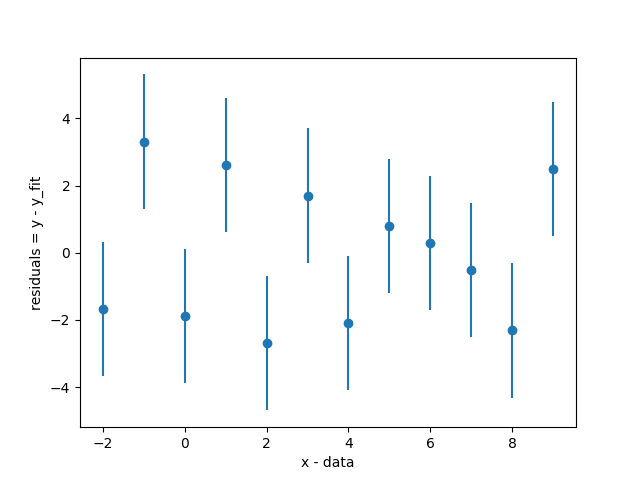
\includegraphics[width=6cm,
        height=6cm]{/home/jp/kod/py/bin/venv/py3/phx444/data_analysis/figures/629.png}
        % Create a subtitle for the figure.
        \caption{Plotting the Residuals}
        % Define the label of the figure. It's good to use 'fig:title', so you know that the label belongs to a figure.
        \label{fig:fig_20}
        \end{center}
\end{figure}


\subsubsection{The last Hoorah}
The final exercise in this week's lab is to deliberately fit an incorrect
function to our points and then use the residuals and some intuition to fix the
problem. If we assign 'wrongfit' as we are instructed

\begin{center}
\begin{minipage}[t]{.75\textwidth}
\begin{lstlisting}[frame=tlrb]
wrongfit = 10.5 * x - 7.2
wrong_r_i = y - wrongfit
\end{lstlisting}
\end{minipage}
\end{center}
Then we get a rather unfortunate plot for the residuals:
\begin{figure}[H]
        % Center the figure.
        \begin{center}
        % Include the eps file, scale it such that it's width equals the column width. You can also put width=8cm for example...
        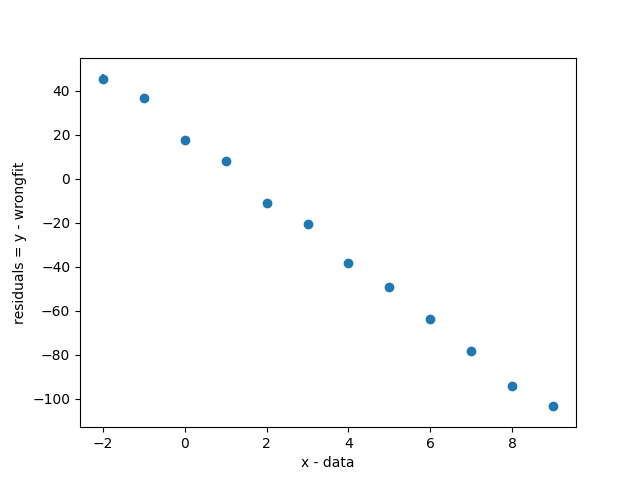
\includegraphics[width=6cm,
        height=6cm]{/home/jp/kod/py/bin/venv/py3/phx444/data_analysis/figures/6210a.png}
        % Create a subtitle for the figure.
        \caption{Plotting the funky residuals}
        % Define the label of the figure. It's good to use 'fig:title', so you know that the label belongs to a figure.
        \label{fig:fig_21}
        \end{center}
\end{figure}

We know that there is a problem because the residuals are not clustered around
zedro. In fact, we can't even see the error bars. Error bar visibility in the
residuals is a great sanity check on a model.The easiest way to correct this
is to re-fit the curve. IE we know that we can get back to the original
distribution by: y = wrong\_r\_i + wrongfit. So, first do this, then fit the curve.
Then plot the fixed curve's residuals and see if they make more sense.

\begin{center}
\begin{minipage}[t]{.75\textwidth}
    \begin{verbatim}
original_distribution = wrong_r_i + wrongfit

re_popt, re_pcov = \
    curve_fit(func_to_fit, x, original_distribution,
                             sigma=y_err, p0=None)

y_re_fit = func_to_fit(x, *popt)

fixed_r_i = y - y_re_fit
\end{verbatim}
\end{minipage}
\end{center}

Fortunately, when we plot the new model, everything seems to be working just
fine:
\begin{figure}[H]
        % Center the figure.
        \begin{center}
        % Include the eps file, scale it such that it's width equals the column width. You can also put width=8cm for example...
        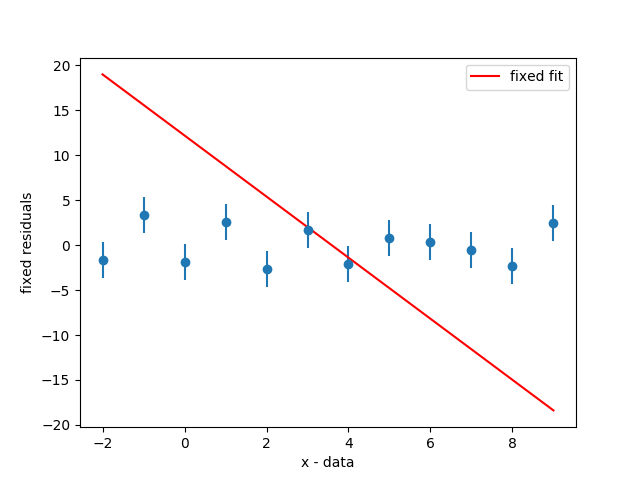
\includegraphics[width=6cm,
        height=6cm]{/home/jp/kod/py/bin/venv/py3/phx444/data_analysis/figures/6210b.png}
        % Create a subtitle for the figure.
        \caption{Plotting the fixed residuals}
        % Define the label of the figure. It's good to use 'fig:title', so you know that the label belongs to a figure.
        \label{fig:fig_22}
        \end{center}
\end{figure}
We can see the error bars! And we know from the previous sections that we've
gotten back to 'normal.' That's really great news, because it means that I can
go to sleep.

\section{Conclusion}
I love data science. Even if I come off as dry and sarcastic on paper,
there is genuinely nothing that I would rather be up doing until \st{12:46AM}
11:59PM on a given night. I'm really excited for this semester and hope that
there continues to be a focus on learning / utilizing the classic Python
libraries!
\end{document}
